\documentclass[20pt]{extarticle}
\usepackage[dvips]{graphicx}

\usepackage{mathtools}

\usepackage{geometry}
	\geometry{
	left=3mm,
	right=3mm,
	top=3mm,
	bottom=9mm,
	includefoot,
	footskip=5mm
	}

\usepackage{amssymb,amsmath}

\renewcommand{\labelitemii}{$\blacktriangleright$}

\usepackage{bm}
\usepackage{color}

\usepackage{esvect}

\usepackage{supertabular}
\usepackage{multirow}
\usepackage{bigstrut}

\usepackage{ulem}
\newcommand{\del}[1]{\textcolor{red}{\sout{#1}}}
\newcommand{\ms}[1]{\textcolor{orange}{\bf [Michiko: #1]}}
\newcommand{\add}[1]{\textcolor{blue}{#1}}
\newcommand{\addd}[1]{\textcolor{orange}{#1}}
\newcommand{\naoki}[1]{\textcolor{green}{\bf [Naoki: #1]}}
\newcommand{\tw}[1]{\textcolor{cyan}{\bf [Takamitsu: #1]}}

\usepackage[hidelinks]{hyperref}
\newcommand{\hrefc}[2]{\href{#1}{\textcolor{blue}{#2}}}

\newcommand{\topdir}{../../..}

% Page number: bottom right, small font, on every page (incl. title page).
\usepackage{fancyhdr}
\pagestyle{fancy}
\fancyhf{}
\renewcommand{\headrulewidth}{0pt}
\renewcommand{\footrulewidth}{0pt}
\fancyfoot[R]{\footnotesize\thepage}
\fancypagestyle{plain}{%
	\fancyhf{}%
	\renewcommand{\headrulewidth}{0pt}%
	\renewcommand{\footrulewidth}{0pt}%
	\fancyfoot[R]{\footnotesize\thepage}%
}

\sloppy

\begin{document}

\title{MATH 463 Mathematical Biology\\ lecture notes\\
6. Data-driven discovery of dynamical systems}
\date{\today}
\author{Naoki Masuda}

\maketitle

\subsection*{Model-driven versus data-driven modeling}

\begin{itemize}
%
\item So far, our modeling workflow has been:
	\begin{enumerate}
	\item The phenomenon or data we want to model are given (e.g., population growth under harvesting).
	\item Build an ODE model, exploiting general knowledge (e.g., exponential growth, logistic growth, mass action, etc.) and/or domain-specific knowledge, if any.
	\item Analyze the constructed ODE model numerically and analytically (if possible).
		\begin{itemize}
		\item Perhaps adjust the parameter values to fit the given data better.
		\end{itemize}
	\item May use the constructed ODE model for prediction, alerting, etc.
	\end{enumerate}
\item This approach may be biased and may not fully exploit the power of data.
%
\end{itemize}

\subsubsection*{Data-driven approach}

\begin{enumerate}
\item We have a $d$-dimensional time series data of length $T$.
	\begin{itemize}
	\item We do not (or pretend not to) know the ODE model.
	\end{itemize}
\item Estimate a $d$-dimensional dynamical system ($=$ ODE system) that matches the given time series data in some sense.
\item Analyze the constructed ODE model.
\item May use the constructed ODE model for prediction, alerting, control, scenario testing, etc.
\end{enumerate}

\subsection*{SINDy (sparse identification of nonlinear dynamics)}

Original paper: \hrefc{https://www.doi.org/10.1073/pnas.1517384113}{Brunton, Proctor \& Kutz, PNAS, 113, 3932 (2016)}
 
\begin{center}
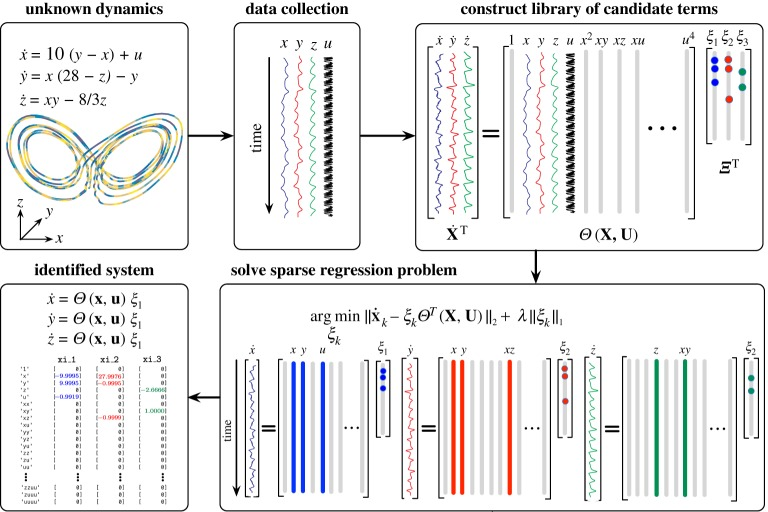
\includegraphics[width=0.95\textwidth]{figures/6_data-driven-ode/Kaiser2018-sindy-schematic.png}
\end{center}
Figure: SINDy. Figure~3 (cropped) of \hrefc{https://www.doi.org/10.1098/rspa.2018.0335}{Kaiser, Kutz \& Brunton, Proc.\ R.\ Soc.\ A, 474, 20180335 (2018)}, \hrefc{https://creativecommons.org/licenses/by/4.0/}{CC BY 4.0}. The figure is drawn for the version of SINDy that also has a control input $u$; for us, simply ignore $u$ and read $\Theta(X, U)$ as $\Theta(X)$.


\begin{itemize}
\item Key idea: sparsity, i.e., assume a small number of terms on the right-hand sides of the estimated ODEs.
	\begin{itemize}
	\item Why sparse? $\to$ Occam's razor $=$ principle of parsimony.
		\begin{itemize}
		\item Recap: ``Everything should be made as simple as possible, but not simpler.'' (Albert Einstein)
		\end{itemize}
	\end{itemize}
\end{itemize}

\subsubsection*{Formulation}

\begin{itemize}
\item Want to estimate $F$ in
$\displaystyle \frac{\text{d}\vec{x}}{\text{d}t} = F(\vec{x})$,
where $\vec{x}(t) = \begin{pmatrix} x_1 \\ x_2 \\ \vdots \\ x_d \end{pmatrix}$.
%
\item The $T \times d$ data matrix:
\[ X = \begin{pmatrix} x_1(t_1) & x_2(t_1) & \ldots & x_d(t_1) \\
x_1(t_2) & x_2(t_2) & \ldots & x_d(t_2) \\
\vdots & \vdots & \ddots & \vdots \\
x_1(t_T) & x_2(t_T) & \ldots & x_d(t_T)
\end{pmatrix}, \]
where $T$ is the number of data points ($=$ time points).
%
\item A $T\times M$ matrix $\Theta$: \emph{library} of linear and nonlinear functions of $x_1$, $\ldots$, $x_d$.
	\begin{itemize}
	\item Some of them will show up on the right-hand sides of the estimated ODE.
	\item $M$ is the number of functions in the library we consider.
	\end{itemize}
\[ \Theta = \begin{pmatrix} g_1(\vec{x}, t_1) & g_2(\vec{x}, t_1) & \ldots & g_M(\vec{x}, t_1) \\
g_1(\vec{x}, t_2) & g_2(\vec{x}, t_2) & \ldots & g_M(\vec{x}, t_2) \\
\vdots & \vdots & \ddots & \vdots \\
g_1(\vec{x}, t_T) & g_2(\vec{x}, t_T) & \ldots & g_M(\vec{x}, t_T)
\end{pmatrix}. \]
	\begin{itemize}
	\item For example, one function we want to consider for the right-hand side of \emph{any} of
\[
\begin{aligned}
\dot{x}_1 =& \cdots,\\
\dot{x}_2 =& \cdots,\\
\vdots &\\
\dot{x}_d =& \cdots
\end{aligned}
\]
may be $x_1$. Then, the first column of $\Theta$ (essentially, function $g_1$) will be
\[ \begin{pmatrix} x_1(t_1) \\ x_1(t_2) \\ \vdots \\ x_1(t_T) \end{pmatrix}. \]
	\item If we want to also consider $x_1 x_2$, then another column of $\Theta$ will be
\[ \begin{pmatrix} x_1(t_1) x_2(t_1) \\ x_1(t_2) x_2(t_2) \\ \vdots \\ x_1(t_T) x_2(t_T) \end{pmatrix}. \]
	\item We can assume any function such as $\sin(x_3(t))$, $\log(x_4(t))$, $x_1(t) x_5(t)^3$, etc.
	\end{itemize}
%
\item A $M \times d$ \emph{sparse} coefficient matrix we will estimate from data:
\[ \Xi = \begin{pmatrix} \vec{\xi}_1 & \vec{\xi}_2 & \cdots & \vec{\xi}_d \end{pmatrix}, \]
where
\[ \vec{\xi}_i = \begin{pmatrix} \xi_{i}^{(1)} \\ \xi_{i}^{(2)} \\ \vdots \\ \xi_{i}^{(M)} \end{pmatrix} \]
are the coefficients for the right-hand side of the $\dot{x}_i = \cdots$ equation.
	\begin{itemize}
	\item $\xi_i^{(j)}$ is how much the right-hand side of $\dot{x}_i = \cdots$ uses the $j$th function in the library.
	\end{itemize}
%
\item Our estimated ODE is determined from
\[ \dot{X} = \Theta \Xi, \]
where
\[ \dot{X} = \begin{pmatrix} \dot{x}_1(t_1) & \dot{x}_2(t_1) & \ldots & \dot{x}_d(t_1) \\
\dot{x}_1(t_2) & \dot{x}_2(t_2) & \ldots & \dot{x}_d(t_2) \\
\vdots & \vdots & \ddots & \vdots \\
\dot{x}_1(t_T) & \dot{x}_2(t_T) & \ldots & \dot{x}_d(t_T)
\end{pmatrix}. \]
	\begin{itemize}
	\item Note that
		\begin{itemize}
		\item $\dot{X}$ is purely from data.
		\item $\Theta$ is from the library functions evaluated at $t = t_1, \ldots, t_T$.
			\begin{itemize}
			\item So, it is from data $+$ library functions.
			\end{itemize}
		\item We estimate $\Xi$.
		\end{itemize}
	\end{itemize}
\end{itemize}

\subsubsection*{Example}

\begin{itemize}
\item $\vec{x} = \begin{pmatrix} x_1 \\ x_2 \end{pmatrix}, \; T=100, \; g_1 = x_1, \; g_2 = x_2, \; g_3 = x_1^2, \; g_4 = x_1 x_2, \; g_5 = x_2^2$.
\item Then:
	\begin{itemize}
	\item Data matrix $X = \begin{pmatrix} x_1(t_1) & x_2(t_1) \\ x_1(t_2) & x_2(t_2) \\ \vdots & \vdots \\ x_1(t_{100}) & x_2(t_{100}) \end{pmatrix}$.
	\item Library
{\small
\[ \Theta = \begin{pmatrix} x_1(t_1) & x_2(t_1) & x_1(t_1)^2 & x_1(t_1) x_2(t_1) & x_2(t_1)^2 \\
x_1(t_2) & x_2(t_2) & x_1(t_2)^2 & x_1(t_2) x_2(t_2) & x_2(t_2)^2 \\
\vdots & \vdots & \vdots & \vdots & \vdots \\
 x_1(t_{100}) & x_2(t_{100}) & x_1(t_{100})^2 & x_1(t_{100}) x_2(t_{100}) & x_2(t_{100})^2 \end{pmatrix}. \]
}
	\item Coefficient matrix
\[ \Xi =
\begin{pmatrix} \vec{\xi}_1 & \vec{\xi}_2 \end{pmatrix} =
\begin{pmatrix} \xi_{1}^{(1)} & \xi_2^{(1)} \\
\xi_1^{(2)} & \xi_2^{(2)} \\
\xi_1^{(3)} & \xi_2^{(3)} \\
\xi_1^{(4)} & \xi_2^{(4)} \\
\xi_1^{(5)} & \xi_2^{(5)}
\end{pmatrix}. \]
	\end{itemize}
%
\item The first column of $\dot{X} = \Theta \Xi$ reads:
{\footnotesize
\[
\begin{aligned}
\begin{pmatrix} \dot{x}_1(t_1) \\ \dot{x}_1(t_2) \\ \vdots \\ \dot{x}_1(t_{100}) \end{pmatrix} =& \Theta \vec{\xi}_1
=
\begin{pmatrix} x_1(t_1) & x_2(t_1) & x_1(t_1)^2 & x_1(t_1) x_2(t_1) & x_2(t_1)^2 \\
x_1(t_2) & x_2(t_2) & x_1(t_2)^2 & x_1(t_2) x_2(t_2) & x_2(t_2)^2 \\
\vdots & \vdots & \vdots & \vdots & \vdots \\
 x_1(t_{100}) & x_2(t_{100}) & x_1(t_{100})^2 & x_1(t_{100}) x_2(t_{100}) & x_2(t_{100})^2 \end{pmatrix}
\begin{pmatrix}
\xi_1^{(1)} \\ \xi_1^{(2)} \\ \xi_1^{(3)} \\ \xi_1^{(4)} \\ \xi_1^{(5)}
\end{pmatrix}\\
%
=&
\begin{pmatrix}
x_1(t_1) \\ x_1(t_2) \\ \vdots \\ x_1(t_{100})
\end{pmatrix}
\xi_1^{(1)}
+
\begin{pmatrix}
x_2(t_1) \\ x_2(t_2) \\ \vdots \\ x_2(t_{100})
\end{pmatrix}
\xi_1^{(2)}
+
\begin{pmatrix}
x_1(t_1)^2 \\ x_1(t_2)^2 \\ \vdots \\ x_1(t_{100})^2
\end{pmatrix}
\xi_1^{(3)}\\
%
&+
\begin{pmatrix}
x_1(t_1) x_2(t_1) \\ x_1(t_2) x_2(t_2) \\ \vdots \\ x_1(t_{100}) x_2(t_{100})
\end{pmatrix}
\xi_1^{(4)}
%
+
\begin{pmatrix}
x_2(t_1)^2 \\ x_2(t_2)^2 \\ \vdots \\ x_2(t_{100})^2
\end{pmatrix}
\xi_1^{(5)}.
\end{aligned}
\]
}
%
\item So, for example,
	\begin{itemize}
	\item $\xi_1^{(1)}$ represents how much the right-hand side of $\dot{x}_1 = \cdots$ uses $x_1$.
	\item $\xi_1^{(4)}$ represents how much the right-hand side of $\dot{x}_1 = \cdots$ uses $x_1 x_2$.
	\end{itemize}
\end{itemize}

\subsubsection*{Get the model by sparse optimization}

\begin{itemize}
\item Determine the coefficients by a convex ``$\ell_1$-regularized sparse regression'':
\[ \hat{\Xi} = \underset{\Xi}{\operatorname{argmin}} \left\| \Theta \Xi - \dot{X} \right\|_2 + \alpha \left\| \Xi \right\|_1. \]
\item In fact, the different columns of $\Xi$ are independent in the above optimization problem, so we do
\[ \vec{\xi}_i = \underset{\vec{\xi}_i}{\operatorname{argmin}} \left\| \Theta \vec{\xi}_i - \dot{X}_i \right\|_2 + \alpha \left\| \vec{\xi}_i \right\|_1 \]
for each $i$, where $\dot{X}_i$ is the $i$th column of matrix $\dot{X}$.
\item $\alpha$: regularization parameter. A large $\alpha$ promotes sparsity of the estimated model.
	\begin{itemize}
	\item Sparsity means most $\xi_{i}^{(j)}$ values are $0$.
	\end{itemize}
\end{itemize}

\subsubsection*{Application examples}

\begin{center}
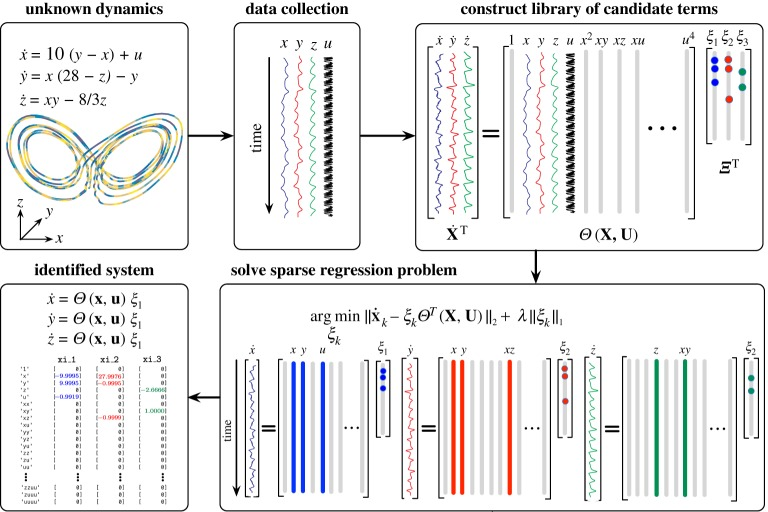
\includegraphics[width=0.95\textwidth]{figures/6_data-driven-ode/Kaiser2018-sindy-schematic.png}
\end{center}
Figure: SINDy (again). Figure~3 (cropped) of \hrefc{https://www.doi.org/10.1098/rspa.2018.0335}{Kaiser, Kutz \& Brunton, Proc.\ R.\ Soc.\ A, 474, 20180335 (2018)}, \hrefc{https://creativecommons.org/licenses/by/4.0/}{CC BY 4.0}.

\begin{center}
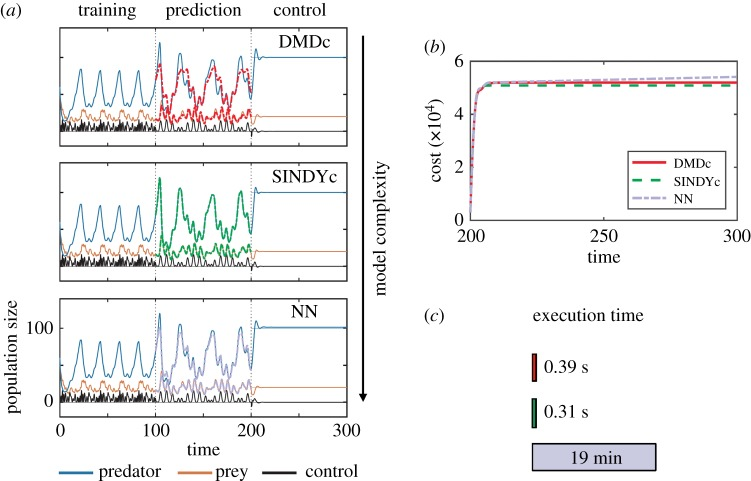
\includegraphics[width=0.8\textwidth]{figures/6_data-driven-ode/Kaiser2018-predator-prey.jpg}
\end{center}
Figure: Another example: Lotka--Volterra. A SINDy model (SINDYc, green), a linear model (DMDc, red), and a neural network (NN, purple) are trained on the same data and then used to predict and to control the system. Figure~5 of \hrefc{https://www.doi.org/10.1098/rspa.2018.0335}{Kaiser, Kutz \& Brunton, Proc.\ R.\ Soc.\ A, 474, 20180335 (2018)}, \hrefc{https://creativecommons.org/licenses/by/4.0/}{CC BY 4.0}.

\begin{center}
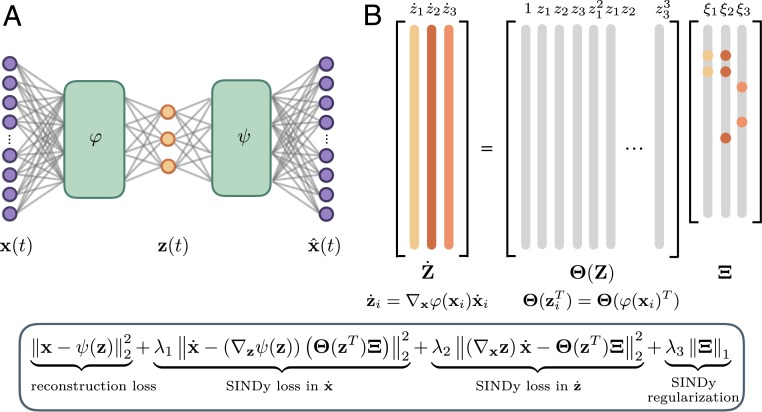
\includegraphics[width=0.8\textwidth]{figures/6_data-driven-ode/Champion2019-sindy-autoencoder.jpg}
\end{center}
Figure: SINDy autoencoder: a neural network first finds a small number of coordinates $\bm z(t)$ from high-dimensional data $\bm x(t)$, and SINDy finds a sparse ODE in those coordinates. Figure~1 of \hrefc{https://www.doi.org/10.1073/pnas.1906995116}{Champion, Lusch, Kutz \& Brunton, PNAS, 116, 22445 (2019)}, \hrefc{https://creativecommons.org/licenses/by/4.0/}{CC BY 4.0}.

\begin{itemize}
\item \hrefc{https://pysindy.readthedocs.io/en/latest/examples/sindy-addl-examples/eba3fdb/example.html}{One more example from physics.}
\end{itemize}

\subsubsection*{Code}

\begin{itemize}
\item \hrefc{https://pysindy.readthedocs.io/en/latest/index.html}{PySINDy}
\item \hrefc{https://github.com/dynamicslab/SINDy-PI?tab=readme-ov-file}{SINDy-PI}
\item \hrefc{https://faculty.washington.edu/kutz/page26/}{MATLAB SINDy code base}
\end{itemize}

\subsubsection*{Tutorials}

\begin{itemize}
\item Various extensions: e.g., partial differential equations.
\item Many tutorials.
	\begin{itemize}
	\item E.g., \hrefc{https://faculty.washington.edu/kutz/}{Nathan Kutz' (University of Washington) website has a lot.}
	\end{itemize}
\item Also see section 7.3 of \hrefc{https://www.cambridge.org/highereducation/books/data-driven-science-and-engineering/6F9A730B7A9A9F43F68CF21A24BEC339\#overview}{Brunton \& Kutz, Data-Driven Science and Engineering (Second Edition), Cambridge University Press (2022).}
\end{itemize}

\subsection*{Application 1: Discovering epidemic models from historical data}

\begin{itemize}
\item Paper: \hrefc{https://doi.org/10.1038/s41598-020-63877-w}{Horrocks \& Bauch, Scientific Reports, 10, 7061 (2020)}.
\item \textbf{Question:} Could an algorithm discover the SIR model from epidemic data alone?
\item Data: weekly \emph{case notifications} (the number of newly reported cases each week) for three childhood infections before mass vaccination:
	\begin{itemize}
	\item measles, England and Wales, 1948--1967,
	\item chickenpox (varicella), Ontario, 1946--1967,
	\item rubella, Ontario, 1946--1960.
	\end{itemize}
\begin{center}
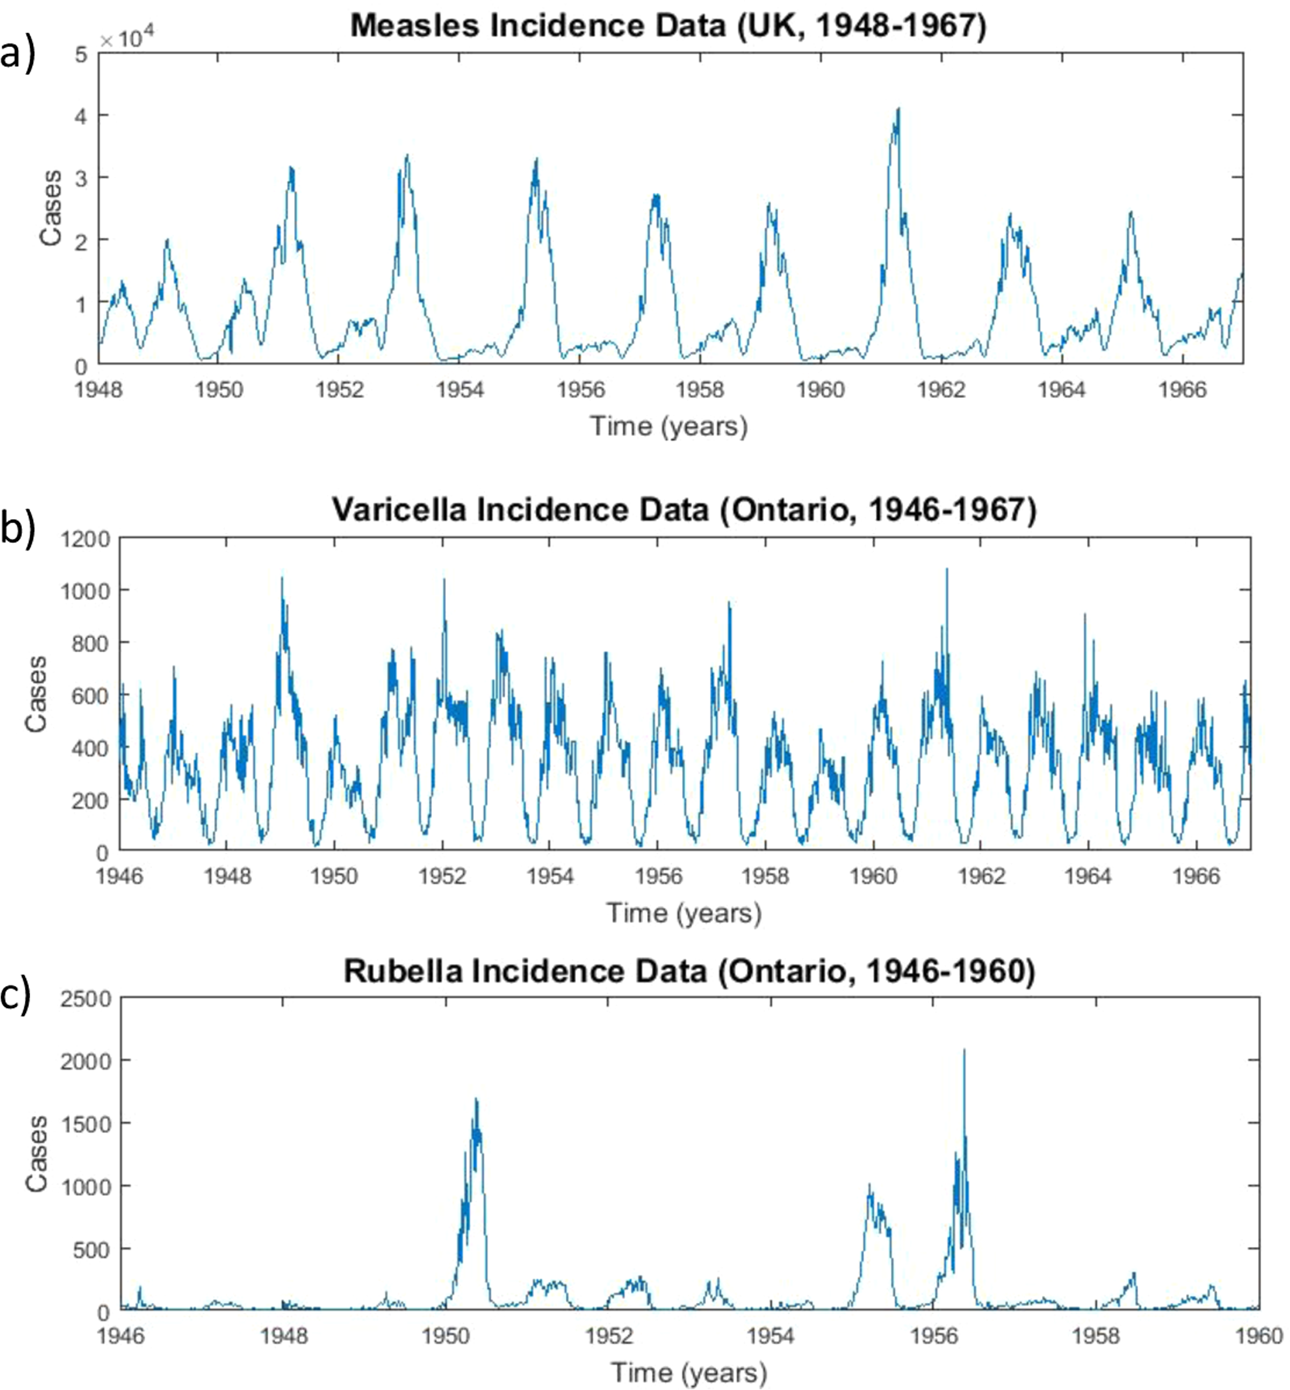
\includegraphics[width=0.62\textwidth]{figures/6_data-driven-ode/Horrocks2020-data.png}\\
\end{center}
Figure: Case notifications for (a) measles, (b) chickenpox, and (c) rubella. Figure~1 of \hrefc{https://doi.org/10.1038/s41598-020-63877-w}{Horrocks \& Bauch, Sci Rep, 10, 7061 (2020)}, \hrefc{https://creativecommons.org/licenses/by/4.0/}{CC BY 4.0}.
\item \textbf{Q:} Looking at the data figure, what do you notice about measles versus chickenpox?
\end{itemize}


\subsubsection*{Turning the data into $S(t)$ and $I(t)$}

\begin{itemize}
\item Problem: SINDy needs the \emph{state variables}, but the data give only reported cases, and only a fraction of infections is ever reported.
\item $I(t)$: convert reported incidence (new cases per week) into prevalence (how many are currently infectious) using the mean infectious period ($\approx 2$ weeks) and an assumed reporting fraction.
\item $S(t)$: nobody ever measures the number of susceptible individuals. It is \emph{reconstructed} by bookkeeping,
\[ S_{t+1} = S_t - \alpha_t C_{t} + B_{t-d}, \]
	\begin{itemize}
	\item $C_t =$ the reported cases,
	\item $(\alpha_t)^{-1} =$ the (time-varying) fraction of all cases reported to the data collection agency,
	\item $B_{t-d} =$ the births $d$ weeks earlier (newborns become susceptible).
	\item This is the standard ``susceptible reconstruction'' of epidemiology.
	\item \textbf{Lesson:} data-driven modeling still needs domain knowledge. Deciding \emph{what the variables are} is already modeling.
	\end{itemize}
\item The reconstructed series are then smoothed before numerical differentiation.
	\begin{itemize}
	\item \textbf{Q:} Why is smoothing needed? (Recall that SINDy needs $\dot{X}$, which is estimated from noisy data by numerical differentiation.)
	\end{itemize}
\end{itemize}

\subsubsection*{The library}

\begin{itemize}
\setcounter{MaxMatrixCols}{20}
\item With $d=2$ state variables $S$ and $I$, they used all polynomials up to second order, and then the same terms multiplied by a seasonal factor:
\[ \Theta(X) = \begin{bmatrix} 1 & S & I & S^2 & I^2 & SI & \beta & \beta S & \beta I & \beta S^2 & \beta I^2 & \beta SI \end{bmatrix}, \]
where
\[ \beta(t) = \beta_0 \left[ 1 + \beta_1 \cos\left( \frac{2\pi t}{T} - \phi \right) \right], \qquad T = 1 \text{ year}. \]
	\begin{itemize}
	\item So $M=12$ candidate functions for each of the two equations.
	\item Why a seasonal term? School terms: children mix much more during the school year.
	\item Note that the library \emph{contains} the SIR model ($SI$ and $\beta SI$ are in it), but it also contains 10 other terms that could be chosen instead.
	\end{itemize}
\item Model selection: sweep the sparsity parameter $\lambda$ (and the unknown initial $S_0$), and pick the model with the lowest AIC (Akaike information criterion), which rewards good fit and penalizes the number of terms.
	\begin{itemize}
	\item AIC is a principled version of Occam's razor. It is covered in statistics courses.
	\end{itemize}
\end{itemize}

\subsubsection*{Result}

\begin{figure}[h]
\begin{center}
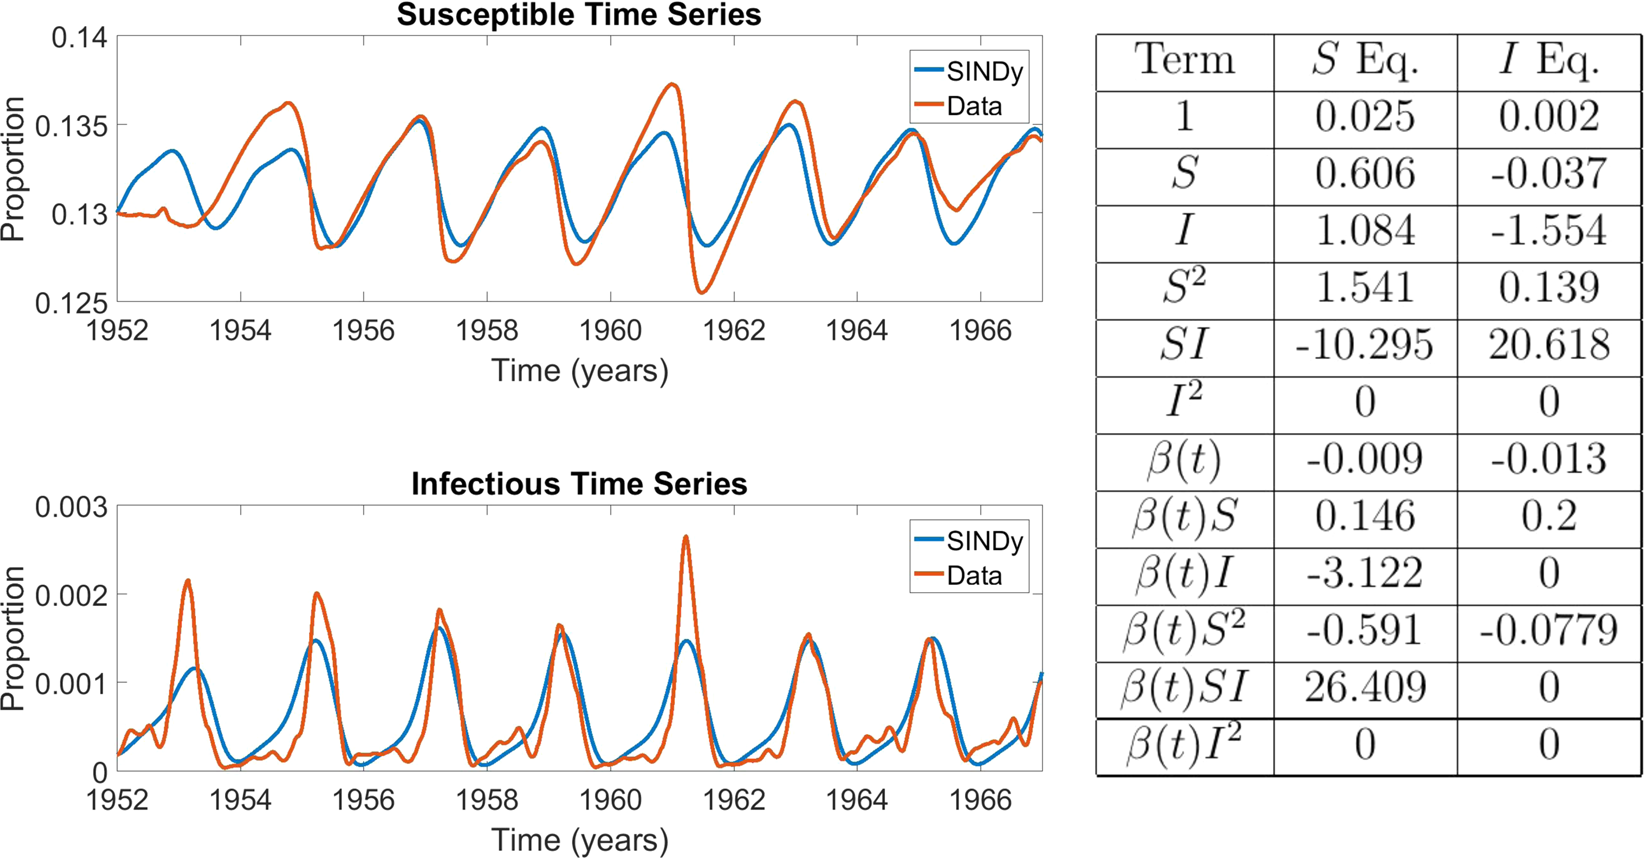
\includegraphics[width=0.95\textwidth]{figures/6_data-driven-ode/Horrocks2020-measles.png}
\caption{Measles: the SINDy-discovered model (blue) against the data (red), and the discovered coefficients. Figure~3 of \hrefc{https://doi.org/10.1038/s41598-020-63877-w}{Horrocks \& Bauch, Sci Rep, 10, 7061 (2020)}, \hrefc{https://creativecommons.org/licenses/by/4.0/}{CC BY 4.0}.}
\end{center}
\end{figure}

\begin{itemize}
\item The discovered model reproduces the \emph{biennial} (two-year) measles cycle.
\item The largest coefficients are those of $SI$ and $\beta(t) SI$, i.e.,
\[ \frac{\text{d}S}{\text{d}t} \approx \cdots - \left[\text{const} + \beta(t)\right] SI, \qquad
\frac{\text{d}I}{\text{d}t} \approx \cdots + \left[\text{const} + \beta(t)\right] SI . \]
	\begin{itemize}
	\item This is \emph{mass-action incidence with a seasonally varying transmission rate}, with the same coefficient appearing with opposite signs in the two equations.
	\item SINDy rediscovered the seasonally forced SIR model that epidemiologists wrote down by hand decades ago.
	\end{itemize}
\item Chickenpox: same conclusion (annual cycle, mass action dominant).
\item Rubella: SINDy failed, returning an annual cycle whereas the data show multi-annual outbreaks. Changing the selection criterion (matching the power spectral density instead of the time series) fixed it.
	\begin{itemize}
	\item Honest reporting of a failure is a good practice.
	\end{itemize}
\end{itemize}

\subsubsection*{Does the discovered model predict something it was not fitted to?}

\begin{itemize}
\item A model that only fits the data it was trained on is of limited interest.
\item Real test: mass vaccination of measles started in the UK in 1968, and the data after that show a \emph{regime shift} from the regular biennial cycle to irregular annual outbreaks.
\item The authors did not refit anything. They took the discovered measles model and simply \emph{reduced the recruitment of susceptible individuals} (which is what vaccination does).
\item The model then produces an annual, irregular cycle: the same transition as in the real post-1968 data.
\end{itemize}

\begin{itemize}
\item \textbf{Take-home messages:}
	\begin{enumerate}
	\item Providing evidence that the theory (or forward modeling) is not arbitrary.
	\item The discovered model extrapolates to a situation it never saw (vaccination), which pure curve fitting would not do.
	\item Data preparation (what are the state variables? how noisy are the derivatives?) and the model selection criterion matter as much as the algorithm.
	\end{enumerate}
\end{itemize}

\subsection*{Application 2: Discovering how CAR T-cells kill cancer cells}

\begin{itemize}
\item Paper: \hrefc{https://doi.org/10.3389/fimmu.2023.1115536}{Brummer, Xella, Woodall, Adhikarla, Cho, Gutova, Brown \& Rockne, Frontiers in Immunology, 14, 1115536 (2023)}.
\item Background: CAR (Chimeric antigen receptor) T-cell therapy takes a patient's T-cells, engineers them to carry a chimeric antigen receptor that recognizes a tumor antigen, and puts them back.
\item \textbf{Question:} what are the \emph{dynamics} of the killing? How does a CAR T-cell's killing rate depend on how many cancer cells are around, and on how many CAR T-cells are around?
	\begin{itemize}
	\item This matters clinically: it determines the dose.
	\end{itemize}
\item Experiment: patient-derived glioblastoma (brain cancer) cells are plated on microelectrodes; the impedance (``cell index'') measures how many cancer cells are attached, every 15 minutes for about a week. CAR T-cells are added at three effector-to-target (E:T) ratios, $1\!:\!4$, $1\!:\!8$, $1\!:\!20$.
\end{itemize}

\begin{figure}[h]
\begin{center}
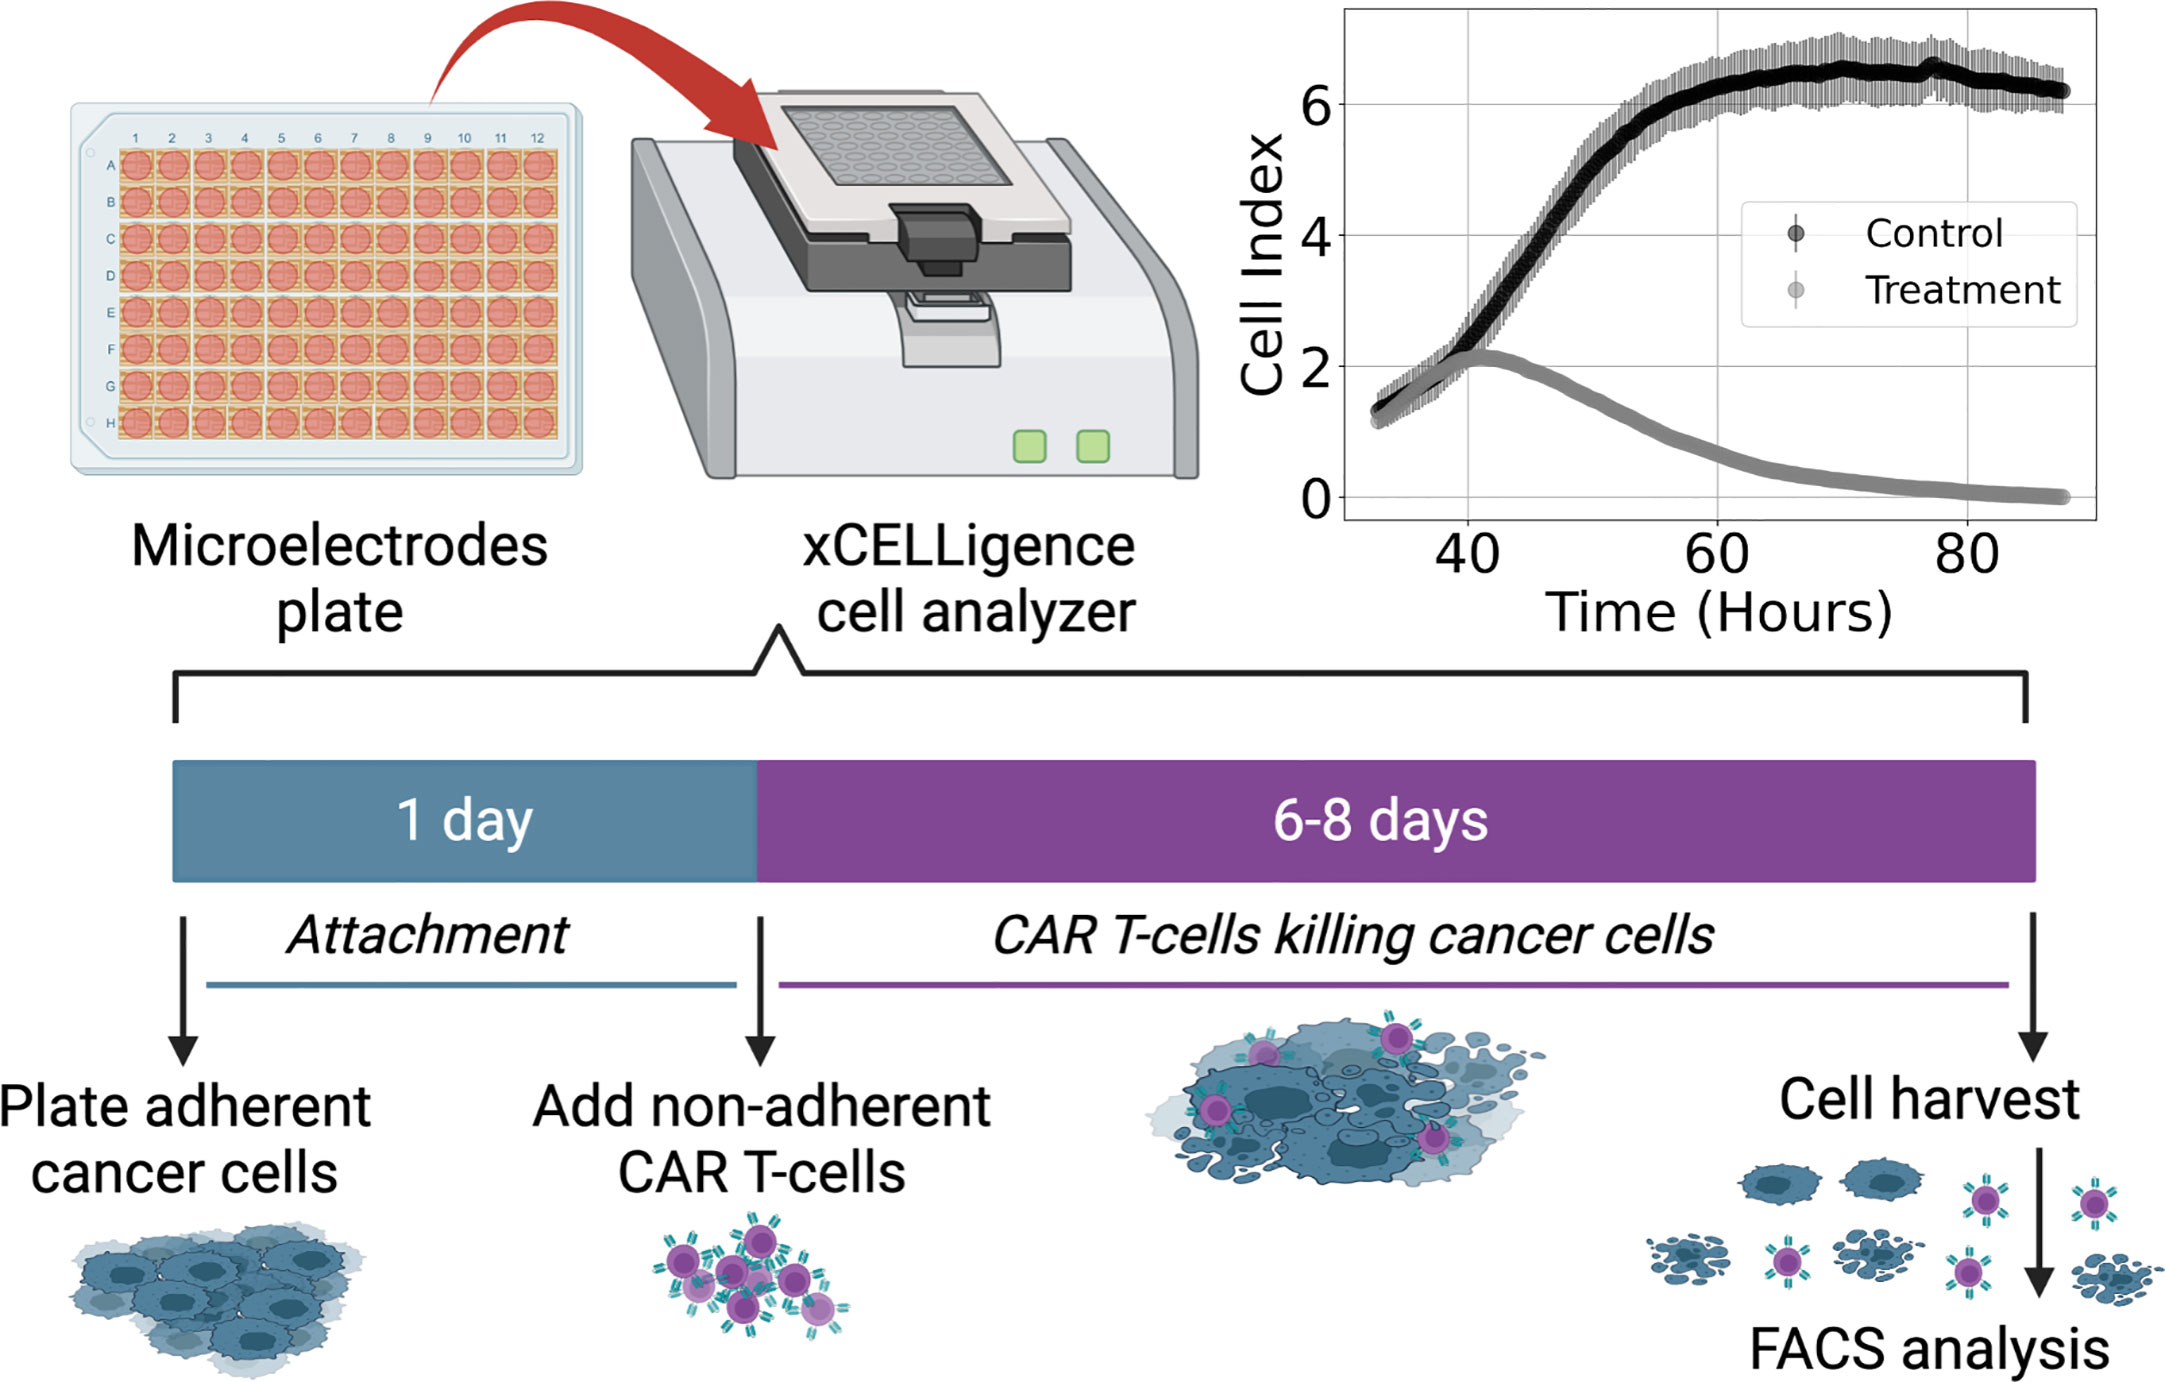
\includegraphics[width=0.8\textwidth]{figures/6_data-driven-ode/Brummer2023-experiment.jpg}
\caption{In vitro killing assay. Cancer cells grow (control, black) until CAR T-cells are added (treatment, gray). Figure~1 of \hrefc{https://doi.org/10.3389/fimmu.2023.1115536}{Brummer et al., Front.\ Immunol., 14, 1115536 (2023)}, \hrefc{https://creativecommons.org/licenses/by/4.0/}{CC BY 4.0}.}
\end{center}
\end{figure}

\subsubsection*{The starting model: predator and prey, again}

\begin{itemize}
\item $x(t)$: cancer cell population.
\item $y(t)$: CAR T-cell population.
\item The standard model in this field is CARRGO (\hrefc{https://doi.org/10.1098/rsif.2019.0734}{Sahoo et al., J R Soc Interface, 17, 20190734 (2020)}):
\[
\begin{aligned}
\frac{\text{d}x}{\text{d}t} =& \rho x \left( 1 - \frac{x}{K} \right) - \kappa_1 x y,\\
\frac{\text{d}y}{\text{d}t} =& \kappa_2 x y - \theta y.
\end{aligned}
\]
	\begin{itemize}
	\item \textbf{Q:} Where have we seen (variants of) this model before?
	\ \\
	\ \\
	\ \\
	\item \textbf{A:} It is Lotka--Volterra with logistic prey (HW2, Problem 2)
		\begin{itemize}
		\item cancer cells are the prey.
		\item CAR T-cells are the predator.
		\end{itemize}
	\item $\rho$: cancer growth rate
	\item $K$: carrying capacity
	\item $\kappa_1$: killing rate
	\item $\kappa_2$: CAR T-cell proliferation per encounter
	\item $\theta$: CAR T-cell death/exhaustion rate.
	\end{itemize}
\item But this model makes three \emph{choices}, each of which could be wrong:
	\begin{enumerate}
	\item the cancer cells grow logistically;
	\item one CAR T-cell binds one cancer cell (``single binding''), giving the mass-action term $xy$;
	\item the killing rate per CAR T-cell is proportional to $x$ (called a Type I functional response).
	\end{enumerate}
\item Idea of the paper: do not choose. Let SINDy $+$ data choose.
\end{itemize}

\subsubsection*{The candidate mechanisms}

\begin{itemize}
\item \textbf{Growth law} $G(x)$: logistic, weak Allee effect, or strong Allee effect (recall section 2).
%
\begin{center}
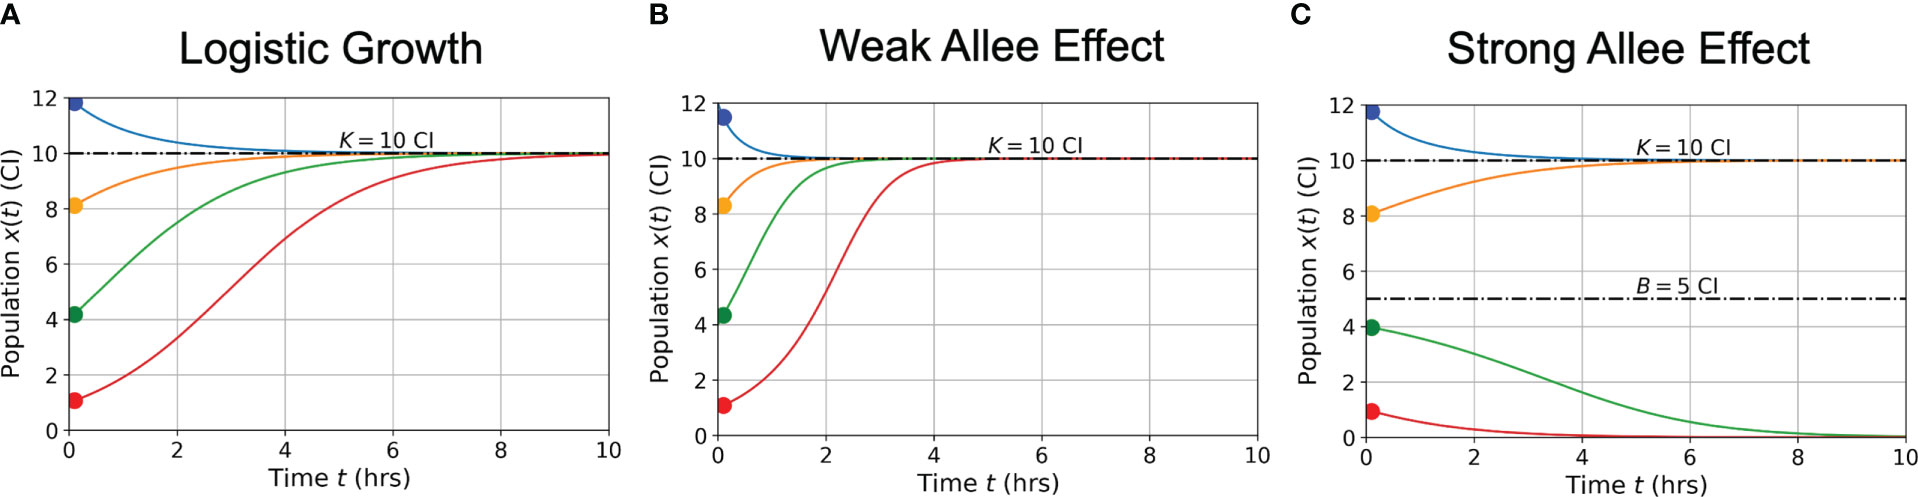
\includegraphics[width=0.9\textwidth]{figures/6_data-driven-ode/Brummer2023-growth.jpg}\\
\end{center}
Figure: Candidate growth laws for the cancer cells. Figure~2 of \hrefc{https://doi.org/10.3389/fimmu.2023.1115536}{Brummer et al., Front.\ Immunol., 14, 1115536 (2023)}, \hrefc{https://creativecommons.org/licenses/by/4.0/}{CC BY 4.0}.
%
\item \textbf{Binding} $\mathcal{B}(y)$: one CAR T-cell per cancer cell, or two (a cancer cell can be attacked by two CAR T-cells at once).
	\begin{itemize}
	\item Single binding gives a term proportional to $y$.
	\item Double binding adds a term proportional to $y^2$.
	\end{itemize}
\item \textbf{Functional response} $\mathcal{R}(x)$: how fast a CAR T-cell responds as a function of how much target is around.
	\begin{itemize}
	\item Type I (linear),
	\item Type II (saturating, fast-to-slow),
	\item Type III (sigmoid, slow-to-fast).
	\item These are the classical Holling functional responses of ecology, applied to immune cells.
	\end{itemize}
\end{itemize}

\begin{figure}[h]
\begin{center}
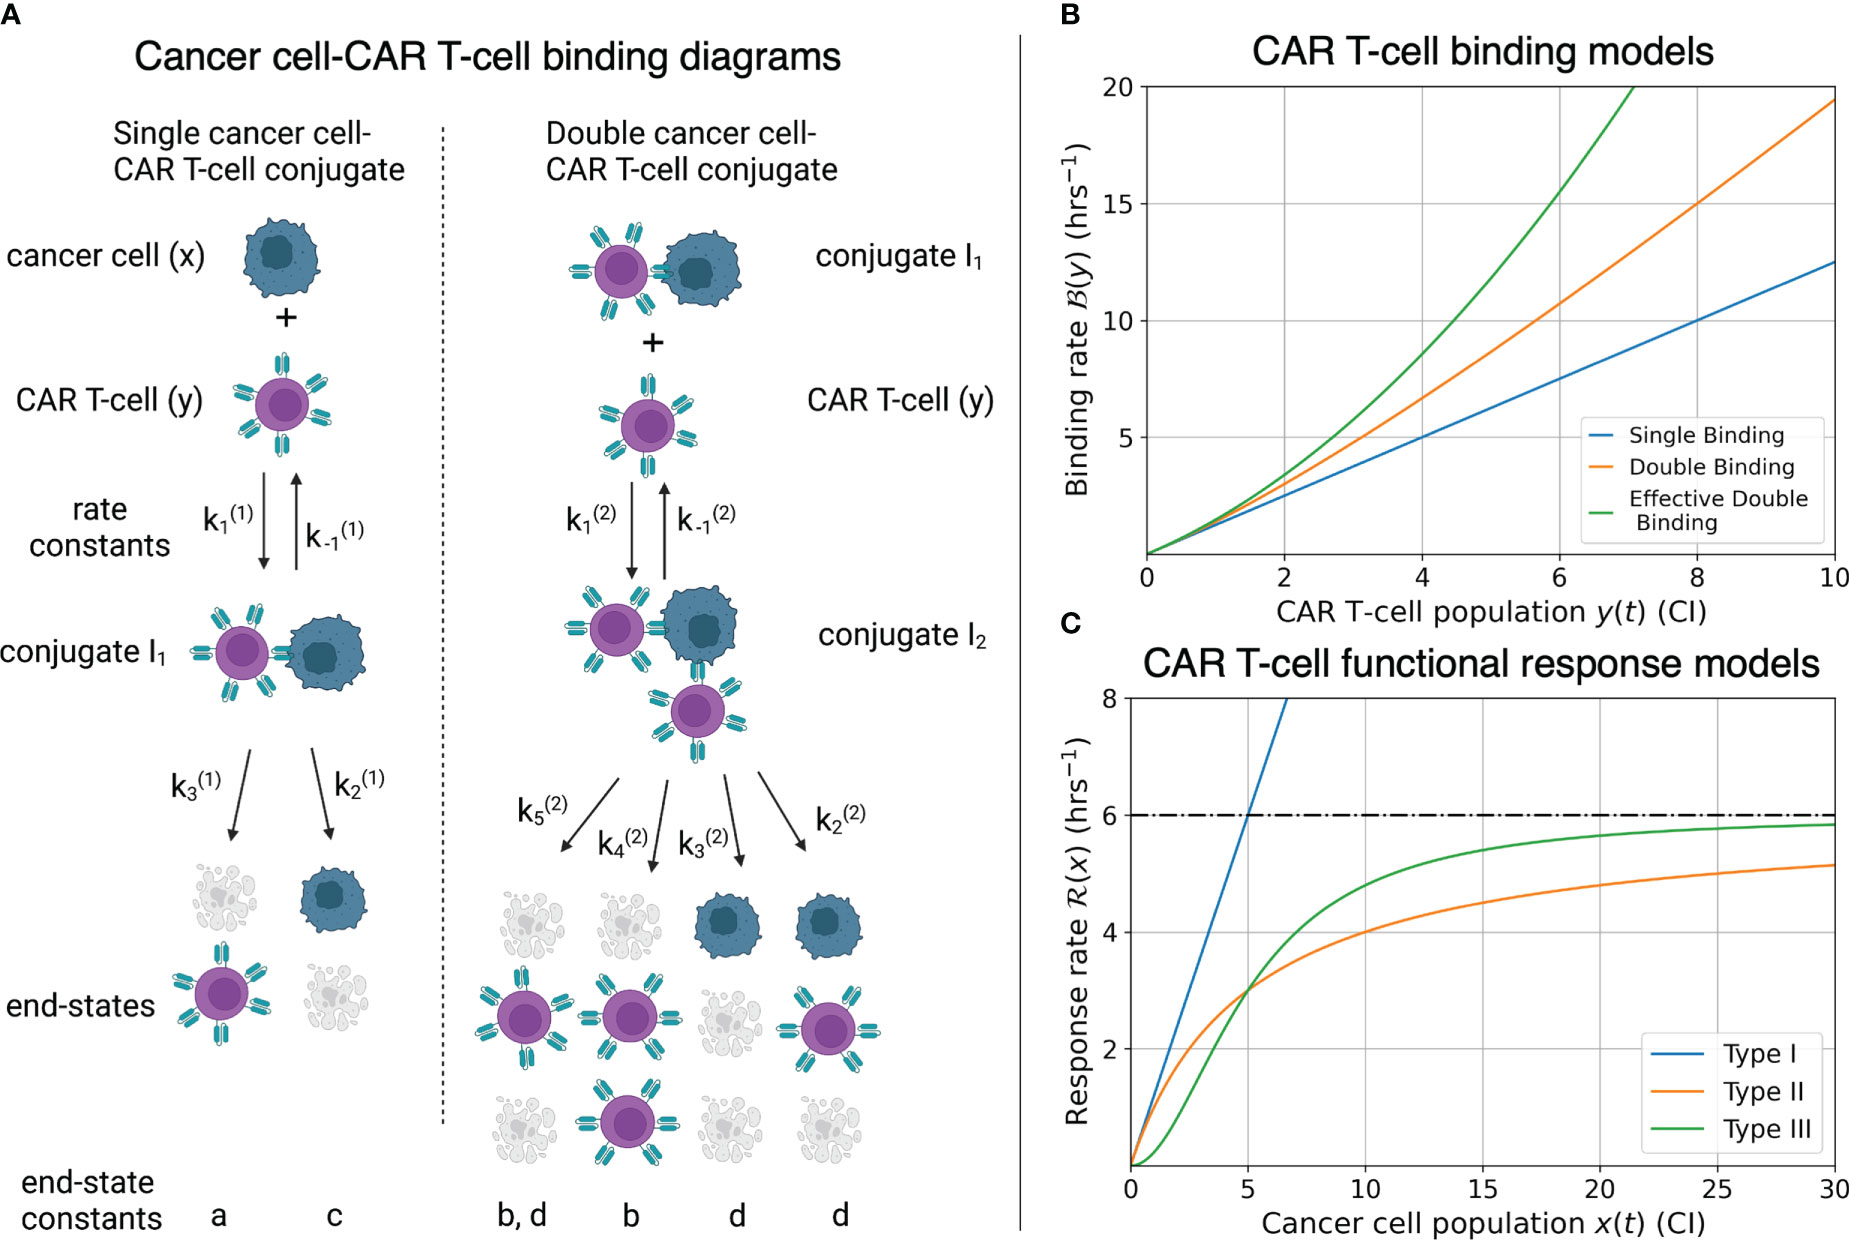
\includegraphics[width=0.95\textwidth]{figures/6_data-driven-ode/Brummer2023-mechanisms.jpg}
\caption{(A) Single versus double cancer cell--CAR T-cell binding. (B) The resulting binding rates as functions of the CAR T-cell population. (C) Type I, II, and III functional responses. Figure~3 of \hrefc{https://doi.org/10.3389/fimmu.2023.1115536}{Brummer et al., Front.\ Immunol., 14, 1115536 (2023)}, \hrefc{https://creativecommons.org/licenses/by/4.0/}{CC BY 4.0}.}
\end{center}
\end{figure}

\begin{itemize}
\item Each combination of (growth law, binding, functional response) corresponds to a specific set of polynomial terms in $x$ and $y$. So the library is
\[ \Theta(X) = \begin{bmatrix} x & y & x^2 & xy & y^2 & x^3 & x^2 y & x y^2 & y^3 \end{bmatrix}. \]
	\begin{itemize}
	\item Sparse regression is being used for \underline{mechanism selection}, not just curve fitting.
	\item They also constrain the signs of the coefficients (e.g., killing must reduce $x$), using biological knowledge.
	\end{itemize}
\end{itemize}

\subsubsection*{Result}

\begin{figure}[h]
\begin{center}
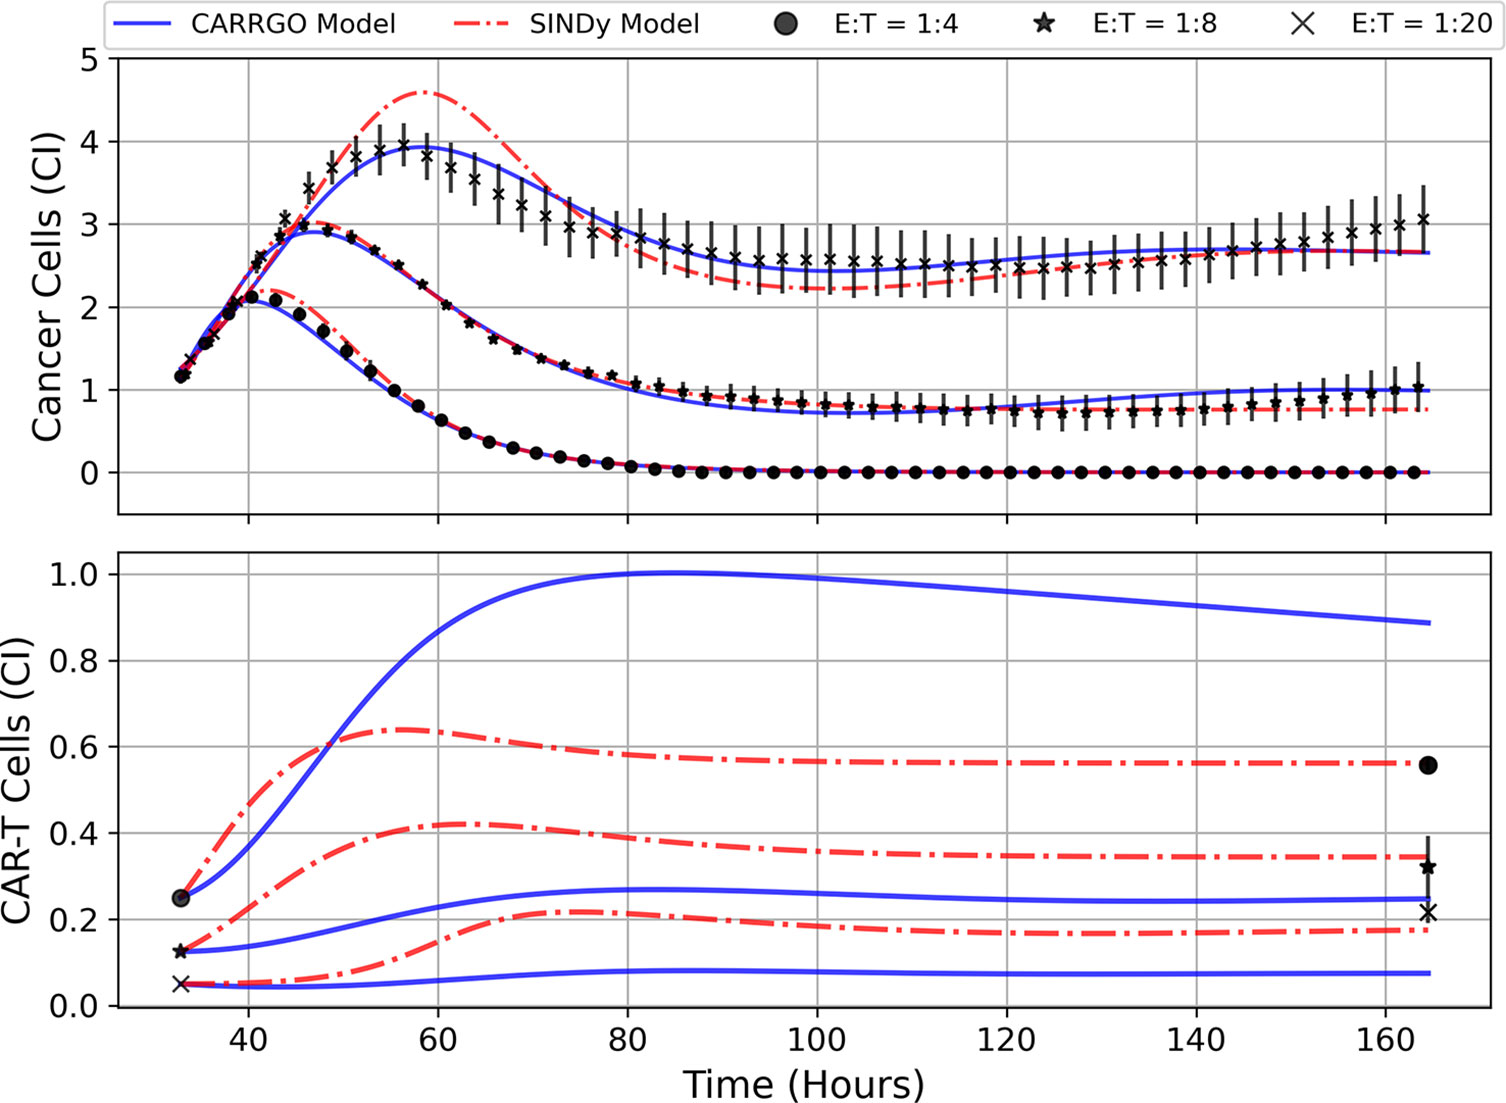
\includegraphics[width=0.72\textwidth]{figures/6_data-driven-ode/Brummer2023-fits.jpg}
\caption{Measured cancer cells (symbols) and the trajectories of the hand-built CARRGO model (blue) and of the SINDy-discovered models (red), for the three E:T ratios. Figure~5 of \hrefc{https://doi.org/10.3389/fimmu.2023.1115536}{Brummer et al., Front.\ Immunol., 14, 1115536 (2023)}, \hrefc{https://creativecommons.org/licenses/by/4.0/}{CC BY 4.0}.}
\end{center}
\end{figure}

\begin{itemize}
\item The discovered models fit about as well as the hand-built CARRGO model, but they are \emph{different models at different doses}:
	\begin{itemize}
	\item E:T $=1:4$ (many CAR T-cells): weak Allee growth, Type II (fast-to-slow) response, \emph{double} binding.
	\item E:T $=1:8$: weak Allee growth, Type II response, \emph{single} binding.
	\item E:T $=1:20$ (few CAR T-cells): logistic growth, Type III (slow-to-fast) response, mixed binding.
	\end{itemize}
\item Biological interpretation: 
	\begin{itemize}
	\item When CAR T-cells are abundant, they gang up on a cancer cell (double binding) and respond most strongly at low tumor burden.
	\item When they are scarce, they attack singly and need a larger tumor burden before responding strongly.
	\end{itemize}
\item That is a hypothesis about \emph{mechanism}, generated by an algorithm, and it is testable in the laboratory.
\item It also implies that the efficacy of the therapy depends on the \emph{ratio} of the two cell populations, not only on the dose of CAR T-cells.
\end{itemize}

\end{document}

